%% AUTO-GENERATED by part2/code/scripts/make_lengthcheck.py from manuscript.tex.
%% Do not edit; regenerate. Two-column journal layout, for page counting only.
\documentclass[9pt,twocolumn,twoside]{opticajnl}
\journal{opticajournal}
\setboolean{shortarticle}{false}
\usepackage{tabularx}
\usepackage{amsmath}
% AUTO-GENERATED by scripts/make_numbers_tex.py -- DO NOT HAND-EDIT.
% Regenerate: python scripts/make_numbers_tex.py
\usepackage{xcolor}  % for the [PENDING] flag color, harmless if already loaded
% \param{...} marks a stated design parameter, as opposed to a result (which
% must be one of the macros below); scripts/check_consistency.py accepts it.
\providecommand{\param}[1]{#1}

\newcommand{\MeasuredContrastTwoX}{2.00}
\newcommand{\KcPredTwoX}{4.22}
\newcommand{\KstarTwoXInterp}{4.18}
\newcommand{\KstarTwoXCI}{none}
\newcommand{\MeanGainTwoX}{0.40}
\newcommand{\MinGainTwoX}{-0.03}
\newcommand{\MeasuredContrastFourX}{3.80}
\newcommand{\KcPredFourX}{6.96}
\newcommand{\KstarFourXInterp}{none}
\newcommand{\KstarFourXCI}{8.98}
\newcommand{\MeanGainFourX}{0.70}
\newcommand{\MinGainFourX}{0.04}
\newcommand{\MeasuredContrastEightX}{5.32}
\newcommand{\KcPredEightX}{9.33}
\newcommand{\KstarEightXInterp}{none}
\newcommand{\KstarEightXCI}{8.98}
\newcommand{\MeanGainEightX}{0.88}
\newcommand{\MinGainEightX}{0.05}
\newcommand{\MinGainAllBudgets}{-0.03}
\newcommand{\SEightGainKLowSlantZero}{0.913}
\newcommand{\SEightLoKLowSlantZero}{0.906}
\newcommand{\SEightHiKLowSlantZero}{0.920}
\newcommand{\SEightGainKLowSlantTwoFive}{3.122}
\newcommand{\SEightLoKLowSlantTwoFive}{3.122}
\newcommand{\SEightHiKLowSlantTwoFive}{3.123}
\newcommand{\SEightGainKLowSlantFive}{2.077}
\newcommand{\SEightLoKLowSlantFive}{2.076}
\newcommand{\SEightHiKLowSlantFive}{2.078}
\newcommand{\SEightGainKLowSlantSevenFive}{0.227}
\newcommand{\SEightLoKLowSlantSevenFive}{0.223}
\newcommand{\SEightHiKLowSlantSevenFive}{0.230}
\newcommand{\SEightGainKLowSlantTen}{0.089}
\newcommand{\SEightLoKLowSlantTen}{0.089}
\newcommand{\SEightHiKLowSlantTen}{0.089}
\newcommand{\SEightGainKLowSlantFifteen}{-0.007}
\newcommand{\SEightLoKLowSlantFifteen}{-0.016}
\newcommand{\SEightHiKLowSlantFifteen}{0.002}
\newcommand{\SEightGainKLowSlantTwenty}{0.024}
\newcommand{\SEightLoKLowSlantTwenty}{0.019}
\newcommand{\SEightHiKLowSlantTwenty}{0.028}
\newcommand{\SEightGainKMidSlantZero}{0.899}
\newcommand{\SEightLoKMidSlantZero}{0.898}
\newcommand{\SEightHiKMidSlantZero}{0.901}
\newcommand{\SEightGainKMidSlantTwoFive}{1.017}
\newcommand{\SEightLoKMidSlantTwoFive}{0.980}
\newcommand{\SEightHiKMidSlantTwoFive}{1.055}
\newcommand{\SEightGainKMidSlantFive}{2.045}
\newcommand{\SEightLoKMidSlantFive}{2.044}
\newcommand{\SEightHiKMidSlantFive}{2.046}
\newcommand{\SEightGainKMidSlantSevenFive}{0.291}
\newcommand{\SEightLoKMidSlantSevenFive}{0.210}
\newcommand{\SEightHiKMidSlantSevenFive}{0.371}
\newcommand{\SEightGainKMidSlantTen}{0.185}
\newcommand{\SEightLoKMidSlantTen}{0.182}
\newcommand{\SEightHiKMidSlantTen}{0.187}
\newcommand{\SEightGainKMidSlantFifteen}{0.046}
\newcommand{\SEightLoKMidSlantFifteen}{0.045}
\newcommand{\SEightHiKMidSlantFifteen}{0.046}
\newcommand{\SEightGainKMidSlantTwenty}{0.011}
\newcommand{\SEightLoKMidSlantTwenty}{0.011}
\newcommand{\SEightHiKMidSlantTwenty}{0.011}
\newcommand{\NZZeroPooledGainThirtyTwo}{0.640}
\newcommand{\NZZeroPooledLoThirtyTwo}{0.640}
\newcommand{\NZZeroPooledHiThirtyTwo}{0.640}
\newcommand{\NZZeroPooledGainOneTwentyEight}{0.641}
\newcommand{\NZZeroPooledLoOneTwentyEight}{0.641}
\newcommand{\NZZeroPooledHiOneTwentyEight}{0.641}
\newcommand{\NZZeroPooledGainTwoFiftySix}{0.645}
\newcommand{\NZZeroPooledLoTwoFiftySix}{0.645}
\newcommand{\NZZeroPooledHiTwoFiftySix}{0.645}
\newcommand{\NZZeroGainKLowThirtyTwo}{1.019}
\newcommand{\NZZeroGainKLowOneTwentyEight}{0.915}
\newcommand{\NZZeroGainKLowTwoFiftySix}{0.894}
\newcommand{\NZZeroGainKMidThirtyTwo}{0.731}
\newcommand{\NZZeroGainKMidOneTwentyEight}{0.900}
\newcommand{\NZZeroGainKMidTwoFiftySix}{0.928}
\newcommand{\SOneBaselineGain}{1.81}
\newcommand{\SOneNoSaturationGain}{2.22}
\newcommand{\SOneNoSaturationRatio}{1.2}
\newcommand{\SOneNoDiffusionRatio}{1.14}
\newcommand{\SOneNoNonlocalityRatio}{0.98}
\newcommand{\SOneNoDyeDepletionRatio}{0.98}
\newcommand{\STwoBaselineGain}{0.11}
\newcommand{\STwoGainMin}{0.08}
\newcommand{\STwoGainMax}{0.15}
\newcommand{\SThreeNominalGain}{1.81}
\newcommand{\SThreeWorstWithinFifty}{1.17}
\newcommand{\SThreeWorstWithinFiftyParam}{dn\_max}
\newcommand{\SThreeBestWithinFifty}{1.92}
\newcommand{\SThreeDnMaxFlipPct}{473}
\newcommand{\SThreeDnMaxWorstGain}{-3.73}
\newcommand{\SThreeDnMaxAtHundred}{0.99}
\newcommand{\SThreeDnMaxMostNegativePct}{-83}
\newcommand{\SThreeDnMaxAtMostNegative}{0.38}
\newcommand{\SThreeDnMaxMostPositivePct}{473}
\newcommand{\SThreeDnMaxAtMostPositive}{-3.73}
\newcommand{\SThreeAnyFlipWithinFifty}{no}
\newcommand{\SATMeanGainTwoX}{0.07}
\newcommand{\SATFracOfMILTwoX}{18}
\newcommand{\SATMeanGainFourX}{0.20}
\newcommand{\SATFracOfMILFourX}{28}
\newcommand{\SATMeanGainEightX}{0.36}
\newcommand{\SATFracOfMILEightX}{42}
\newcommand{\SATFitNRMSE}{0.103}
\newcommand{\SATFitAEff}{7.05}
\newcommand{\SATSubCliffGain}{0.98}
\newcommand{\SATSubCliffMILGain}{1.37}
\newcommand{\SATSubCliffFracOfMIL}{71}
\newcommand{\SATSubCliffFracMin}{79}
\newcommand{\SATSubCliffFracMax}{79}
\newcommand{\SATSubCliffK}{1.31}
\newcommand{\SATNearCliffK}{3.93}
\newcommand{\SATNearCliffFrac}{56}
\newcommand{\SATPostCliffK}{5.24}
\newcommand{\SATPostCliffFracMin}{-28}
\newcommand{\SATPostCliffFracMax}{-28}
\newcommand{\SeedCountMin}{3}
\newcommand{\SeedCountMax}{3}
\newcommand{\SeedCountDesc}{3}
\newcommand{\SeedCountModal}{3}
\newcommand{\SeedCountNExtraConfigs}{0}
\newcommand{\SeedCount}{3}
\newcommand{\NResultFiles}{2279}

% --- supplement macros: gradient check, RCWA ---
\newcommand{\GradCheckMaxRelErr}{6.5\times10^{-6}}
\newcommand{\GradCheckNDirs}{6}
\newcommand{\RCWAMaxDevThreeCase}{0.038}
\newcommand{\RCWAVGridMaxDev}{0.98}
\newcommand{\RCWAVGridNCases}{90}
\newcommand{\RCWAUnslantedMaxDev}{0.29}
\newcommand{\RCWANormalMedianDev}{0.001}

% --- validation (Phase 6 / Section 6) macros ---
\newcommand{\NLiteratureSources}{3}
\newcommand{\NRMSEBruderGrowthDnKExp}{0.28}
\newcommand{\NRMSEBruderGrowthDnKSim}{0.17}
\newcommand{\NRMSEHsiehGrowthDnK}{0.10}
\newcommand{\NRMSEWorstFit}{0.28}
\newcommand{\NRMSEBestFit}{0.10}
\newcommand{\NGoodFits}{3}
\newcommand{\NRMSEWorstInRegime}{0.28}
\newcommand{\NRMSEBestInRegime}{0.17}
\newcommand{\NInRegimeSources}{2}
\newcommand{\BayfolDnMaxRatio}{5.7}

% --- baseline completeness (Sec. 5.2 / F4b) macros ---
\newcommand{\GSGainMin}{-1.27}
\newcommand{\GSGainMax}{0.00}
\newcommand{\LPCGainMin}{-1.82}
\newcommand{\LPCGainMax}{0.07}
\newcommand{\MILGainMinAtTwoX}{-0.03}

% --- shrinkage-induced shift bound (Discussion) macros ---
\newcommand{\ShrinkagePct}{0.5}
\newcommand{\ShrinkageSlantDeg}{20}
\newcommand{\ShrinkageThicknessUm}{30}
\newcommand{\ShrinkageShiftNm}{54.6}
\newcommand{\ShrinkageFracLowK}{1.7}
\newcommand{\ShrinkageFracHighK}{13.7}

% --- cost-benefit (Sec. 5.1) macros ---
\newcommand{\ComputeMatchRatio}{21.7}

% --- R1 reconstruction figure macros ---
\newcommand{\ROneSeedValue}{0}

% --- WP3 baseline (RSGD/GPC, Sec. 5.2) macros ---
\newcommand{\RSGDGainMin}{-0.00}
\newcommand{\RSGDGainMax}{0.00}
\newcommand{\GPCGainMin}{-1.98}
\newcommand{\GPCGainMax}{0.07}
\newcommand{\GPCLPCMaxAbsDiffTwoX}{0.18}

% --- WP4 (target ensemble / noise robustness, Sec. 5.x) macros ---
\newcommand{\SFourGainBarsTwoX}{0.90}
\newcommand{\SFourBootCILoBarsTwoX}{0.90}
\newcommand{\SFourBootCIHiBarsTwoX}{0.90}
\newcommand{\SFourGainBarsEightX}{1.95}
\newcommand{\SFourBootCILoBarsEightX}{1.95}
\newcommand{\SFourBootCIHiBarsEightX}{1.95}
\newcommand{\SFourGainSpotsTwoX}{3.22}
\newcommand{\SFourBootCILoSpotsTwoX}{3.19}
\newcommand{\SFourBootCIHiSpotsTwoX}{3.23}
\newcommand{\SFourGainSpotsEightX}{4.07}
\newcommand{\SFourBootCILoSpotsEightX}{3.99}
\newcommand{\SFourBootCIHiSpotsEightX}{4.12}
\newcommand{\SFourGainRandomBinaryTwoX}{0.17}
\newcommand{\SFourBootCILoRandomBinaryTwoX}{0.17}
\newcommand{\SFourBootCIHiRandomBinaryTwoX}{0.17}
\newcommand{\SFourGainRandomBinaryEightX}{0.24}
\newcommand{\SFourBootCILoRandomBinaryEightX}{0.24}
\newcommand{\SFourBootCIHiRandomBinaryEightX}{0.24}
\newcommand{\SFiveNoiseStdPct}{5}
\newcommand{\SFiveNoiselessGain}{0.90}
\newcommand{\SFiveNoisyGain}{0.88}

% --- WP5 (joint miscalibration Monte Carlo, Sec. 5.x) macros ---
\newcommand{\SSixNDraws}{30}
\newcommand{\SSixMeanGain}{1.76}
\newcommand{\SSixBootCILo}{1.73}
\newcommand{\SSixBootCIHi}{1.79}
\newcommand{\SSixNNegative}{0}
\newcommand{\SSixWorstDrawGain}{1.61}
\newcommand{\SSixBestDrawGain}{1.94}
\newcommand{\SSixPctRange}{25}

% --- WP6 (depth-resolved absorption, Sec. 5.x) macros ---
\newcommand{\SSevenGainODZero}{1.81}
\newcommand{\SSevenGainODOneTenth}{1.51}
\newcommand{\SSevenGainODThreeTenths}{1.45}

% --- main grid (complete M1 cells only), ablations, twin fits ---
\newcommand{\MOneNK}{10}
\newcommand{\MOneNCells}{30}
\newcommand{\MOneKMin}{1.96}
\newcommand{\MOneKMax}{15.71}
\newcommand{\MOneKList}{1.96, 2.62, 3.49, 3.93, 4.19, 4.83, 5.71, 6.98, 8.98, 15.71}
\newcommand{\MOneNPositive}{29}
\newcommand{\MOneNCIAboveZero}{27}
\newcommand{\MOneNCIIncludesZero}{2}
\newcommand{\MOneNNegative}{1}
\newcommand{\MOneNegK}{4.19}
\newcommand{\MOneNegBudget}{2}
\newcommand{\MOneNegGain}{-0.03}
\newcommand{\MOneNegCILo}{-0.05}
\newcommand{\MOneNegCIHi}{-0.005}
\newcommand{\MaxGainTwoX}{1.42}
\newcommand{\MaxGainKTwoX}{2.62}
\newcommand{\GainHighKTwoX}{0.01}
\newcommand{\GainHighKLoTwoX}{0.002}
\newcommand{\GainHighKHiTwoX}{0.008}
\newcommand{\MaxGainFourX}{2.13}
\newcommand{\MaxGainKFourX}{1.96}
\newcommand{\GainHighKFourX}{0.04}
\newcommand{\GainHighKLoFourX}{0.009}
\newcommand{\GainHighKHiFourX}{0.062}
\newcommand{\MaxGainEightX}{2.52}
\newcommand{\MaxGainKEightX}{2.62}
\newcommand{\GainHighKEightX}{0.05}
\newcommand{\GainHighKLoEightX}{0.019}
\newcommand{\GainHighKHiEightX}{0.091}
\newcommand{\MOneNExcluded}{0}
\newcommand{\SOneGBaselineSub}{4.41}
\newcommand{\SOneGBaselineNear}{0.90}
\newcommand{\SOneGBaselinePost}{0.11}
\newcommand{\SOneGNoSatSub}{5.39}
\newcommand{\SOneGNoSatNear}{0.61}
\newcommand{\SOneGNoSatPost}{0.66}
\newcommand{\SOneGNoDiffSub}{4.93}
\newcommand{\SOneGNoDiffNear}{1.14}
\newcommand{\SOneGNoDiffPost}{0.10}
\newcommand{\SOneGNoNonlocSub}{4.47}
\newcommand{\SOneGNoNonlocNear}{0.82}
\newcommand{\SOneGNoNonlocPost}{0.05}
\newcommand{\SOneGNoDyeSub}{4.36}
\newcommand{\SOneGNoDyeNear}{0.84}
\newcommand{\SOneGNoDyePost}{0.11}
\newcommand{\SOneKSub}{1.31}
\newcommand{\SOneKNear}{3.93}
\newcommand{\SOneKPost}{5.24}
\newcommand{\SXGBaselineSub}{4.41}
\newcommand{\SXNBaselineSub}{3}
\newcommand{\SXGBaselineNear}{0.90}
\newcommand{\SXNBaselineNear}{3}
\newcommand{\SXGBaselinePost}{0.11}
\newcommand{\SXNBaselinePost}{3}
\newcommand{\SXGNoMonomerSub}{-0.12}
\newcommand{\SXNNoMonomerSub}{3}
\newcommand{\SXGNoMonomerNear}{-0.09}
\newcommand{\SXNNoMonomerNear}{3}
\newcommand{\SXGNoMonomerPost}{-0.08}
\newcommand{\SXNNoMonomerPost}{3}
\newcommand{\SXGNoDyeSub}{4.35}
\newcommand{\SXNNoDyeSub}{3}
\newcommand{\SXGNoDyeNear}{0.84}
\newcommand{\SXNNoDyeNear}{3}
\newcommand{\SXGNoDyePost}{0.11}
\newcommand{\SXNNoDyePost}{3}
\newcommand{\SXGNoSatSub}{5.38}
\newcommand{\SXNNoSatSub}{3}
\newcommand{\SXGNoSatNear}{0.62}
\newcommand{\SXNNoSatNear}{3}
\newcommand{\SXGNoSatPost}{0.66}
\newcommand{\SXNNoSatPost}{3}
\newcommand{\SXGOnlyTanhSub}{-0.10}
\newcommand{\SXNOnlyTanhSub}{3}
\newcommand{\SXGOnlyTanhNear}{-0.02}
\newcommand{\SXNOnlyTanhNear}{3}
\newcommand{\SXGOnlyTanhPost}{-0.03}
\newcommand{\SXNOnlyTanhPost}{3}
\newcommand{\SXGOnlyDyeSub}{14.37}
\newcommand{\SXNOnlyDyeSub}{3}
\newcommand{\SXGOnlyDyeNear}{6.38}
\newcommand{\SXNOnlyDyeNear}{3}
\newcommand{\SXGOnlyDyePost}{7.40}
\newcommand{\SXNOnlyDyePost}{3}
\newcommand{\SXGOnlyMonomerSub}{5.75}
\newcommand{\SXNOnlyMonomerSub}{3}
\newcommand{\SXGOnlyMonomerNear}{1.73}
\newcommand{\SXNOnlyMonomerNear}{3}
\newcommand{\SXGOnlyMonomerPost}{1.26}
\newcommand{\SXNOnlyMonomerPost}{3}
\newcommand{\SXGLinearSub}{14.94}
\newcommand{\SXNLinearSub}{3}
\newcommand{\SXGLinearNear}{7.66}
\newcommand{\SXNLinearNear}{3}
\newcommand{\SXGLinearPost}{9.04}
\newcommand{\SXNLinearPost}{3}
\newcommand{\SXGLinearMatchedSub}{-0.00}
\newcommand{\SXNLinearMatchedSub}{3}
\newcommand{\SXGLinearMatchedNear}{0.00}
\newcommand{\SXNLinearMatchedNear}{3}
\newcommand{\SXGLinearMatchedPost}{0.10}
\newcommand{\SXNLinearMatchedPost}{3}
\newcommand{\SXGNoMonomerMatchedSub}{3.64}
\newcommand{\SXNNoMonomerMatchedSub}{3}
\newcommand{\SXGNoMonomerMatchedNear}{0.72}
\newcommand{\SXNNoMonomerMatchedNear}{3}
\newcommand{\SXGNoMonomerMatchedPost}{0.08}
\newcommand{\SXNNoMonomerMatchedPost}{3}
\newcommand{\SXGOnlyDyeMatchedSub}{1.98}
\newcommand{\SXNOnlyDyeMatchedSub}{3}
\newcommand{\SXGOnlyDyeMatchedNear}{0.42}
\newcommand{\SXNOnlyDyeMatchedNear}{3}
\newcommand{\SXGOnlyDyeMatchedPost}{-0.02}
\newcommand{\SXNOnlyDyeMatchedPost}{3}
\newcommand{\SXGOnlyTanhMatchedSub}{2.80}
\newcommand{\SXNOnlyTanhMatchedSub}{3}
\newcommand{\SXGOnlyTanhMatchedNear}{0.53}
\newcommand{\SXNOnlyTanhMatchedNear}{3}
\newcommand{\SXGOnlyTanhMatchedPost}{0.12}
\newcommand{\SXNOnlyTanhMatchedPost}{3}
\newcommand{\SXDeviceMaxDiff}{0.001}
\newcommand{\SATFracLowKMin}{36}
\newcommand{\SATFracLowKMax}{44}
\newcommand{\SATFracSecondKMin}{53}
\newcommand{\SATFracSecondKMax}{66}
\newcommand{\SATNBelowBSGD}{12}
\newcommand{\SATNCells}{29}
\newcommand{\SThreeDnMaxAtMinusFifty}{1.17}
\newcommand{\SThreeDnMaxAtPlusFifty}{1.66}
\newcommand{\MTwoRGainSub}{3.19}
\newcommand{\MTwoRLoSub}{2.94}
\newcommand{\MTwoRHiSub}{3.43}
\newcommand{\MTwoRGainNear}{0.81}
\newcommand{\MTwoRLoNear}{0.81}
\newcommand{\MTwoRHiNear}{0.81}
\newcommand{\MTwoRGainPost}{0.12}
\newcommand{\MTwoRLoPost}{0.12}
\newcommand{\MTwoRHiPost}{0.13}
\newcommand{\MTwoRSATFracSub}{79}
\newcommand{\MTwoRSATFracNear}{56}
\newcommand{\MTwoRSATFracPost}{-28}
\newcommand{\HoldoutASimIn}{0.17}
\newcommand{\HoldoutASimOut}{0.48}
\newcommand{\HoldoutASimKbleach}{0.2}
\newcommand{\HoldoutASimDnMax}{0.0504}
\newcommand{\HoldoutASimAtBound}{none}
\newcommand{\HoldoutAExpIn}{0.28}
\newcommand{\HoldoutAExpOut}{1.09}
\newcommand{\HoldoutAExpKbleach}{0.2}
\newcommand{\HoldoutAExpDnMax}{0.289}
\newcommand{\HoldoutAExpAtBound}{none}
\newcommand{\HoldoutBSimIn}{0.02}
\newcommand{\HoldoutBSimOut}{0.40}
\newcommand{\HoldoutBSimKbleach}{0.0667}
\newcommand{\HoldoutBSimDnMax}{0.0418}
\newcommand{\HoldoutBSimAtBound}{none}
\newcommand{\HoldoutBExpIn}{0.17}
\newcommand{\HoldoutBExpOut}{0.31}
\newcommand{\HoldoutBExpKbleach}{0.0215}
\newcommand{\HoldoutBExpDnMax}{0.0321}
\newcommand{\HoldoutBExpAtBound}{none}

% ---- Applied Optics additions: sensitivity and slant boundary ----
\newcommand{\SensNominalGain}{1.81}
\newcommand{\SensRangeDZero}{0.19}
\newcommand{\SensWorstDZero}{1.73}
\newcommand{\SensWorstPctDZero}{50}
\newcommand{\SensRangeSigma}{0.06}
\newcommand{\SensWorstSigma}{1.76}
\newcommand{\SensWorstPctSigma}{-50}
\newcommand{\SensRangeKappa}{0.19}
\newcommand{\SensWorstKappa}{1.68}
\newcommand{\SensWorstPctKappa}{-50}
\newcommand{\SensRangeDnMax}{0.64}
\newcommand{\SensWorstDnMax}{1.17}
\newcommand{\SensWorstPctDnMax}{-50}
\newcommand{\SensRankOne}{$\Delta n_{\max}$}
\newcommand{\SensRankTwo}{$\kappa$}
\newcommand{\SensRankThree}{$D_0$}
\newcommand{\SensRankFour}{$\sigma$}
\newcommand{\SensTopRangeRatio}{3.4}
\newcommand{\SensRSquared}{0.88}
\newcommand{\SensNDraws}{30}
\newcommand{\SensBetaDZero}{-0.019}
\newcommand{\SensBetaLoDZero}{-0.031}
\newcommand{\SensBetaHiDZero}{-0.007}
\newcommand{\SensBetaSigma}{+0.010}
\newcommand{\SensBetaLoSigma}{-0.003}
\newcommand{\SensBetaHiSigma}{+0.027}
\newcommand{\SensBetaKappa}{+0.024}
\newcommand{\SensBetaLoKappa}{+0.013}
\newcommand{\SensBetaHiKappa}{+0.034}
\newcommand{\SensBetaDnMax}{+0.071}
\newcommand{\SensBetaLoDnMax}{+0.054}
\newcommand{\SensBetaHiDnMax}{+0.090}
\newcommand{\SensNResolved}{3}
\newcommand{\RCWASlantNCases}{336}
\newcommand{\RCWASlantOnsetDeg}{2.5}
\newcommand{\RCWASlantFirstZero}{0.460}
\newcommand{\RCWASlantZerothZero}{0.44}
\newcommand{\RCWASlantDevZero}{0.05}
\newcommand{\RCWASlantFirstTwoFive}{0.023}
\newcommand{\RCWASlantZerothTwoFive}{0.85}
\newcommand{\RCWASlantDevTwoFive}{0.41}
\newcommand{\RCWASlantFirstFive}{0.018}
\newcommand{\RCWASlantZerothFive}{0.85}
\newcommand{\RCWASlantDevFive}{0.51}
\newcommand{\RCWASlantFirstSevenFive}{0.014}
\newcommand{\RCWASlantZerothSevenFive}{0.89}
\newcommand{\RCWASlantDevSevenFive}{0.52}
\newcommand{\RCWASlantFirstTen}{0.005}
\newcommand{\RCWASlantZerothTen}{0.88}
\newcommand{\RCWASlantDevTen}{0.52}
\newcommand{\RCWASlantFirstFifteen}{0.001}
\newcommand{\RCWASlantZerothFifteen}{0.90}
\newcommand{\RCWASlantDevFifteen}{0.52}
\newcommand{\RCWASlantFirstTwenty}{0.002}
\newcommand{\RCWASlantZerothTwenty}{0.91}
\newcommand{\RCWASlantDevTwenty}{0.53}
\newcommand{\SlantCollapseDeg}{7.5}
\newcommand{\SlantMaxGainBeyondCollapse}{0.29}
\newcommand{\SlantCollapseThreshDB}{0.5}

% --- diffraction-efficiency confirmation (Sec. 5.1) macros ---
\newcommand{\DEMeanGainTwoX}{1.80}
\newcommand{\DEMeanGainFourX}{3.00}
\newcommand{\DEMeanGainEightX}{3.94}
\newcommand{\DEMinGainAllBudgets}{-0.251}
\newcommand{\DENNegative}{15}
\newcommand{\DENPairs}{90}

% --- wasted-media measurement (Sec. 5.4) macros ---
\newcommand{\WastedMediaThreshDB}{2}
\newcommand{\WastedMediaBSGDFrac}{37}
\newcommand{\WastedMediaMILFrac}{0}
\newcommand{\WastedMediaBSGDFracOneDB}{60}
\newcommand{\WastedMediaMILFracOneDB}{57}
\newcommand{\WastedMediaBSGDFracThreeDB}{17}
\newcommand{\WastedMediaMILFracThreeDB}{0}
\newcommand{\WastedMediaNConfigs}{30}
\newcommand{\WastedMediaGSFrac}{53}
\newcommand{\WastedMediaGSFracOneDB}{60}
\newcommand{\WastedMediaGSFracThreeDB}{33}
\newcommand{\WastedMediaLPCFrac}{47}
\newcommand{\WastedMediaLPCFracOneDB}{60}
\newcommand{\WastedMediaLPCFracThreeDB}{33}
\newcommand{\WastedMediaSATFrac}{33}
\newcommand{\WastedMediaSATFracOneDB}{60}
\newcommand{\WastedMediaSATFracThreeDB}{0}
\newcommand{\WastedMediaRSGDFrac}{37}
\newcommand{\WastedMediaRSGDFracOneDB}{60}
\newcommand{\WastedMediaRSGDFracThreeDB}{17}
\newcommand{\WastedMediaGPCFrac}{47}
\newcommand{\WastedMediaGPCFracOneDB}{60}
\newcommand{\WastedMediaGPCFracThreeDB}{30}


\begin{document}

\title{Media-in-the-loop holography: designing photopolymer exposures through a
differentiable recording model}

\author[1,*]{Chaitanya Tripathi}
\affil[1]{Ashoka University, Rajiv Gandhi Education City, Sonipat, Haryana 131029, India. \href{https://orcid.org/0009-0002-4094-0323}{ORCID 0009-0002-4094-0323}}
\affil[*]{chaitanya.tripathi\_ug2025@ashoka.edu.in}

\begin{abstract}
A write-once volume photopolymer must be exposed before the medium distorts the
target, and the error is measurable only once it is permanent. We optimize the
exposure through a differentiable recording model: non-local
polymerization-driven diffusion read out by beam propagation. Over
\MOneNCells{} spatial-frequency and contrast-budget cells the designed exposure
beats a media-blind optimizer in \MOneNPositive{}, by up to
\MaxGainEightX\,dB, and removes every exposure falling more than
\WastedMediaThreshDB\,dB short of an oracle reference. The gain needs a
nonlinear dose response, depends most on the index budget, and vanishes once
the fringes tilt. We give the calibration measurements required and when not to
use the method.
\end{abstract}

\maketitle


\section{Introduction}
A laboratory recording a volume hologram in a photopolymer faces a question
that computer-generated holography on a spatial light modulator does not. The
medium is written once. Whatever the exposure delivers is what the material
keeps, and the reconstruction error can be measured only after it is permanent.
Three practical questions follow. When is it worth designing the exposure
through a model of the recording, rather than treating the medium as a linear
transfer? When does that design stop helping? And what must be measured to
calibrate the model before trusting it? This paper answers all three for one
medium family, in simulation, and reports the boundary of each answer.

On a rewritable modulator the corresponding problem is solved by measurement.
Camera-in-the-loop (CITL) optimization records the reconstruction and
back-propagates the residual into the display
model~\cite{peng2020neural}; related approaches refine the model with
Wirtinger gradients~\cite{chakravarthula2019wirtinger}, learned
proxies~\cite{shi2021towards} or time-multiplexed
control~\cite{choi2022time}. Every one of them needs to rewrite the modulator
and try again.

Volume photopolymers such as Bayfol HX~\cite{bruder2017bayfol},
acrylamide/PVA and PQ/PMMA~\cite{hsieh2022pqpmma} record a permanent index
distribution through photopolymerization and mass transport, and the recorded
index is not a scaled copy of the exposure: monomer
diffusion~\cite{zhao1994diffusion,sheridan2012reply}, non-local chain
growth~\cite{sheridan2000nonlocal,gleeson2008chain}, dye bleaching and a
saturating index response act nonlinearly~\cite{kowalski2016design}. A
CITL-style measurement therefore arrives too late, and the recording model has
to carry the correction with no feedback at all.

Differentiable models of a fabrication process already sit inside optical
design loops: neural lithography learns a photolithography simulator for
diffractive optics~\cite{zheng2023neural}, and adjoint inverse design treats a
physical forward model as a differentiable layer~\cite{hughes2018adjoint}.
Concurrently, Wechsler et
al.~\cite{wechsler2026shvam} coupled a differentiable wave-optical model to a
photochemical model for holographic volumetric printing and demonstrated
printed parts, an experiment this study does not attempt; we make no priority
claim for differentiable recording models in a design loop.

What this paper adds is a characterization, with the numbers a laboratory would
need before committing material. We measure how much an exposure optimized
through a differentiable recording model (``media-in-the-loop'', MIL) improves
on the same optimizer run with a linear, media-blind recording assumption, and
then map where that improvement lives: across spatial frequency and contrast
budget (Section~\ref{sec:gain}), against a reference that says how much of the
achievable quality is being thrown away (Section~\ref{sec:failure-rate}),
across the recording mechanisms that could be responsible
(Section~\ref{sec:mechanism}), and against fringe slant, where it stops
(Section~\ref{sec:slant}). Section~\ref{sec:sensitivity} ranks the model
parameters by how much the design gain depends on getting each one right, and
Section~\ref{sec:guidelines} turns that ranking into a calibration protocol:
which measurements are needed, in what order, and when to leave the method
alone.

The recording model (non-local polymerization-driven diffusion, NPDD), the
readout (split-step beam propagation) and the optimizer are all established;
the contribution is their combination into an exposure-design loop and its
characterization. Every headline number is a paired difference (MIL minus
media-blind design) with both arms designed and scored on the same simulated
medium, the ``twin''. An exposure-independent calibration error of the twin
cancels in that difference; an exposure-dependent one does not, so we also
design on the nominal twin and record on miscalibrated ones
(Sections~\ref{sec:robustness} and~\ref{sec:sensitivity}) and compare the twin
with published data (Section~\ref{sec:twin-validation}). All results are
simulation outputs of this study unless cited, and every number is generated by
script from released per-job result files. This is the second part of a
two-part study; Part~1 characterized phase-only CGH degradation with idealized
modulators~\cite{tripathi2025holoforge}.

\section{Model}
\label{sec:model}
Table~\ref{tab:mediumparams} lists every constant; the released code is the
reference implementation.

\subsection{Exposure and feasible set}
\label{sec:model-exposure}
The design variable is the delivered exposure $E(x)\ge 0$ on the transverse
coordinate $x$, constrained to a mean dose $E_0$ and a peak-to-mean contrast
budget $B_c$:
\begin{equation}
\label{eq:feasible-set}
\mathcal{E}(E_0,B_c)=\Big\{E:\;E\ge0,\;\overline{E}=E_0,\;
\max_x E(x)/\overline{E}\le B_c\Big\}.
\end{equation}
$B_c$ is the quantity a recording setup actually controls, through the fringe
visibility and the beam ratio. After every optimizer step the exposure is
projected onto $\mathcal{E}$ by 20 alternating passes of dose rescaling,
$E\leftarrow E\,E_0/(\overline{E}+\epsilon)$, and peak clipping,
$E\leftarrow\min(E,B_cE_0)$. Both operations are elementwise and
differentiable; the residual relative constraint violation after 20 passes is
below $10^{-6}$ on the tested targets.

\subsection{Recording: non-local polymerization-driven diffusion}
\label{sec:model-npdd}
Free monomer $u(x,t)$ ($u(x,0)=1$), polymer $N(x,t)$ ($N(x,0)=0$) and
unbleached dye $d(x,t)$ ($d(x,0)=1$) evolve as in the NPDD
model~\cite{sheridan2000nonlocal}, itself built on the local model of Zhao and
Mouroulis~\cite{zhao1994diffusion}:
\begin{align}
\partial_t u &= \partial_x\!\big(D_{\text{eff}}(N)\,\partial_x u\big) - G_\sigma*(F u), \label{eq:npdd-u}\\
\partial_t N &= G_\sigma*(F u), \label{eq:npdd-N}\\
\partial_t d &= -k_{\text{bleach}}\,I\,d, \label{eq:npdd-d}
\end{align}
with $F=\kappa\,(I d)^\gamma$, recording intensity $I\propto E$, a Gaussian
non-local kernel $G_\sigma$ of width $\sigma$
($\widehat{G_\sigma}(K)=e^{-K^2\sigma^2/2}$) and
$D_{\text{eff}}(N)=D_0e^{-\alpha_D N}$. The kernel acts on the production term
$Fu$, so that polymer initiated at $x'$ is deposited at
$x$~\cite{sheridan2000nonlocal}. The recorded index modulation is
\begin{equation}
\label{eq:npdd-dn}
\Delta n(x)=\Delta n_{\max}\tanh\!\big(\beta N(x)\big),\qquad \beta=1.5 .
\end{equation}
The saturating map and the value of $\beta$ are modelling choices of this
work, held fixed in every fit. Three mechanisms saturate the dose response:
monomer depletion ($u\to0$), dye bleaching ($d\to0$) and the $\tanh$ map;
Section~\ref{sec:mechanism} separates them.

\subsection{Small-signal transfer function and a first design rule}
\label{sec:model-mtf}
Before any optimization, the recording equations already say roughly where
designing through them can help. Take $I(x)=I_{\text{mean}}(1+m\cos Kx)$ with
$m\ll1$, neglect dye depletion ($d\approx1$) and hold
$D_{\text{eff}}=D_0$, so that Eqs.~\eqref{eq:npdd-u}--\eqref{eq:npdd-d} are
linearized about the start of recording. The uniform fields obey
$\dot u_0=-F_0u_0$ with $F_0=\kappa I_{\text{mean}}^\gamma$, and eliminating
the first-order Fourier component quasi-statically gives
\begin{equation}
\label{eq:hk}
H(K)=\frac{\exp(-K^2\sigma^2/2)}{1+D_0K^2/F_0}.
\end{equation}
Non-locality rolls the recorded modulation off as a Gaussian in $K\sigma$ and
diffusion as a Lorentzian in $K\sqrt{D_0/F_0}$. Undoing that roll-off asks for
a pre-boost $1/H(K)$ of the target's spatial-frequency content, and the
contrast budget caps how much pre-boost an exposure can carry: beyond some
$K_c(B_c)$ the required boost exceeds the realizable contrast, and the
heuristic predicts the advantage should change sign there.

Equation~\eqref{eq:hk} is a motivating argument, not a validated transfer
function. It does not match the full simulator, while an independent numerical
linearization of the same equations does (Supplement 1, Section S1). It is used
here only to place the $K_c$ markers in Fig.~\ref{fig:gain}(a) and to define
the linear pre-compensation baseline of Section~\ref{sec:method}; no result
depends on its being exact, and Section~\ref{sec:gain} reports where the data
depart from it.

\subsection{Integration and gradients}
\label{sec:model-imex}
Equations~\eqref{eq:npdd-u}--\eqref{eq:npdd-d} are integrated over
$t_{\text{total}}=10$\,s in $n_{\text{steps}}=300$ first-order
implicit--explicit steps. The explicit reaction step evaluates the non-local
production by fast Fourier transform, caps consumed monomer at the monomer
available (so $u\ge0$ and $u+N$ is conserved to rounding error) and updates $d$
exactly for fixed $I$. The implicit diffusion step applies
$\exp(-\bar{D}K^2\,\mathrm{d}t)$ in Fourier space with $\bar{D}$ the spatial
mean of $D_{\text{eff}}$; this approximation to Eq.~\eqref{eq:npdd-u} has a
one-step error of about $0.1\%$ of the scale of $u$ at a representative late
state, and its accumulation over a trajectory was not bounded. Gradients are
the discrete adjoint of this integrator, obtained by reverse-mode automatic
differentiation~\cite{griewank2008evaluating,paszke2019pytorch}, and agree with
central finite differences to a maximum relative error of
$\GradCheckMaxRelErr$ over \GradCheckNDirs{} random directions through the full
chain (Supplement 1, Section S10).

\subsection{Readout: split-step beam propagation}
\label{sec:model-readout}
The recorded profile $\Delta n(x)$ is extruded uniformly through a slab of
thickness $T$ and read out at wavelength $\lambda$ by scalar split-step beam
propagation~\cite{feit1978light}: $n_z=128$ slices, each applying the phase
$\exp[ik_0\Delta n\,\mathrm{d}z(1-s)]$ ($k_0=2\pi/\lambda$, shrinkage $s$)
followed by band-limited angular-spectrum propagation~\cite{goodman2005fourier},
then one angular-spectrum step to the reconstruction plane, where the
intensity is the reconstruction $R$. The periodic window represents an
infinite grating. Slanted fringes ($x-z\tan\phi=\text{const}$) are
represented by a per-slice lateral Fourier shift. All headline results use an
unslanted grating ($\phi=0$), the geometry in which scalar theory is closest
to rigorous coupled-wave analysis (RCWA)~\cite{moharam1981rigorous}
(Section~\ref{sec:slant}). Between $n_z=128$ and $256$ the paired gain changes
from \NZZeroGainKLowOneTwentyEight{} to \NZZeroGainKLowTwoFiftySix\,dB at
$K=1.96$\,rad/\textmu m and from \NZZeroGainKMidOneTwentyEight{} to
\NZZeroGainKMidTwoFiftySix\,dB at $K=\SOneKNear$\,rad/\textmu m (one seed,
Supplement 1, Section S3). The Klein--Cook parameter
$Q=2\pi\lambda T/(n_0\Lambda^2)$, $\Lambda=2\pi/K$~\cite{klein1967unified},
crosses 10 at $K\approx2.79$\,rad/\textmu m, so the two lowest tested $K$ lie
in the intermediate regime. Kogelnik theory~\cite{kogelnik1969coupled} is used
only as a closed-form cross-check.

\subsection{Loss and optimizer}
\label{sec:model-loss}
With target intensity $I_t$ on $n_x$ samples, the loss is the scale-invariant
mean-squared error
\begin{equation}
\label{eq:si-mse}
\mathcal{L}(R,I_t)=\frac{1}{n_x}\big\|\alpha^\star R-I_t\big\|_2^2\big/\max(I_t)^2,\qquad
\alpha^\star=\langle R,I_t\rangle/\langle R,R\rangle,
\end{equation}
and we report $\mathrm{PSNR}_{\text{si}}=-10\log_{10}\mathcal{L}$, a monotone
transform of the optimized objective. The optimizer is
Adam~\cite{kingma2015adam} (learning rate $5\times10^{-2}$, 800 iterations,
convergence tolerance $10^{-4}$) on the parameterization
$E=\mathrm{softplus}(\theta)+10^{-6}$. The random seed enters only through the
initialization $\theta_0=10^{-2}z$, $z\sim\mathcal{N}(0,I)$, so seed-to-seed
spread measures sensitivity to the starting point, not model or parameter
uncertainty.

\begin{table}[!htbp]
\centering
\caption{Default medium and simulation parameters. Medium values are
illustrative acrylamide/PVA-like choices inside cited ranges, not a refit of
one published medium.}
\label{tab:mediumparams}
\small\renewcommand{\arraystretch}{1.2}
\begin{tabularx}{\linewidth}{l l X}
\hline
Parameter & Default & Source \\
\hline
$D_0$ & $0.1\,\mu\mathrm{m}^2/\mathrm{s}$ & illustrative; AA/PVA literature value $0.01$~\cite{sheridan2012reply} \\
$\sigma$ & $0.08\,\mu\mathrm{m}$ & illustrative; literature range $0.01$--$0.04\,\mu\mathrm{m}$~\cite{gleeson2008chain} \\
$\kappa$ & $2.0$ & calibration choice (cures the medium to $N\approx1$ at unit dose) \\
$\gamma$ & $1.0$ & within the literature range $0.5$--$1.0$~\cite{sheridan2000nonlocal} \\
$\Delta n_{\max}$ & $3.5\times10^{-3}$ & within the AA/PVA range $1.5$--$5\times10^{-3}$ \\
$k_{\text{bleach}}$, $\alpha_D$ & $0.2$, $1.0$ & order of magnitude, not independently sourced \\
$\beta$ & $1.5$ & shape constant of Eq.~\eqref{eq:npdd-dn} (this work) \\
$s$ & $0.5\%$ & placeholder of typical AA/PVA magnitude \\
$T$, $n_0$, $\lambda$, $\phi$ & $30\,\mu$m, $1.5$, $405$\,nm, $0^\circ$ & operating point; slant swept in Section~\ref{sec:slant} \\
Grid & $n_x=1024$, $\mathrm{d}x=0.05\,\mu$m & $51.2\,\mu$m periodic window; $n_z=128$ \\
\hline
\end{tabularx}
\end{table}

\section{Methods compared and benchmark}
\label{sec:method}
All methods share the exposure parameterization, the projection onto
$\mathcal{E}$ and scoring on the full twin. \textbf{MIL} optimizes
Eq.~\eqref{eq:si-mse} with the twin (NPDD and beam propagation) inside the
loss. \textbf{Media-blind SGD (BSGD)} runs the same optimizer under the linear
recording assumption $\Delta n=\Delta n_{\max}(E-\overline{E})$ without
shrinkage and scores its exposure on the twin; it is the design a laboratory
produces when it treats the medium as a linear transfer, and it is the
reference every gain in this paper is measured against.
\textbf{Gerchberg--Saxton (GS)} is alternating-projection phase
retrieval~\cite{gerchberg1972practical,fienup1982phase}, its phase converted to
an exposure by the same linear assumption. \textbf{Linear pre-compensation
(LPC)} boosts each spatial-frequency component of the target by $1/H(K)$ from
Eq.~\eqref{eq:hk} and then projects, so it is the closed-form use of the
Section~\ref{sec:model-mtf} design rule. \textbf{Gamma pre-compensation (GPC)}
inverts a fitted pointwise saturating map. \textbf{TV-regularized SGD (RSGD)}
is BSGD with a total-variation penalty whose weight was tuned on the twin per
budget; the tuned weight is zero at all three budgets, so RSGD reduces to BSGD.
The \textbf{saturation-only surrogate (SAT)} optimizes against a pointwise
saturating model with all transport removed, calibrated to the twin by one
fitted parameter (NRMSE \SATFitNRMSE); it asks whether a laboratory could skip
the transport physics. The \textbf{constrained oracle (ORC)} optimizes against
an ideal linear medium under the same exposure constraints; it is a
gradient-optimized reference, not a proven bound.

The benchmark target is a binary bar pattern at spatial frequency $K$, with
periods rounded to an even number of pixels so that each nominal $K$ is
rendered exactly. The main grid covers \MOneNK{} spatial frequencies,
$K\in\{\MOneKList\}$\,rad/\textmu m, at budgets $B_c\in\{2,4,8\}$, i.e.\
\MOneNCells{} cells, each with every method complete. Ablation and robustness
studies use $K=\SOneKSub$, \SOneKNear{} and \SOneKPost\,rad/\textmu m at
$B_c=2$. Iterative methods run with three seeds and deterministic ones (GS,
LPC, GPC) once. The paired gain of a cell is the mean over seeds of
$\mathrm{PSNR}_{\text{si}}(\text{MIL})-\mathrm{PSNR}_{\text{si}}(\text{BSGD})$
at equal seed; intervals are two-sided 95\% Student-$t$ intervals over seeds
unless a bootstrap~\cite{efron1993bootstrap} is stated. All simulations ran on
one laptop (NVIDIA RTX 3050 GPU; the factorial, compute-matched and
parameter-sensitivity jobs on its CPU).

\section{Results}
\label{sec:results}

\subsection{Where designing through the model pays off}
\label{sec:gain}
The paired gain is positive in \MOneNPositive{} of \MOneNCells{} cells and its
95\% interval excludes zero in \MOneNCIAboveZero{} (Fig.~\ref{fig:gain}(a)).
The largest cell means are \MaxGainTwoX, \MaxGainFourX{} and
\MaxGainEightX\,dB at $B_c=2$, 4 and 8, all at
$K\le\MaxGainKTwoX$\,rad/\textmu m; the grid means are
\MeanGainTwoX/\MeanGainFourX/\MeanGainEightX\,dB. At the highest tested
$K=\MOneKMax$\,rad/\textmu m the gain is \GainHighKTwoX, \GainHighKFourX{} and
\GainHighKEightX\,dB, which is to say nothing. One cell is negative:
$K=\MOneNegK$\,rad/\textmu m at $B_c=\MOneNegBudget$, \MOneNegGain\,dB (95\%
interval [\MOneNegCILo, \MOneNegCIHi]). The seed intervals are narrow because
the seed changes only the initialization (Sections~\ref{sec:robustness}
and~\ref{sec:sensitivity} treat model error). Diffraction efficiency shows the
same budget ordering (mean paired gain
\DEMeanGainTwoX/\DEMeanGainFourX/\DEMeanGainEightX{} percentage points) but
\DENNegative{} of \DENPairs{} per-seed pairs are negative (minimum
\DEMinGainAllBudgets{} points).

The heuristic of Section~\ref{sec:model-mtf} predicts a sign change at
$K_c=\KcPredTwoX$, \KcPredFourX{} and \KcPredEightX\,rad/\textmu m (dashed
lines in Fig.~\ref{fig:gain}(a)). At $B_c=2$ the gain crosses zero at
$K^*=\KstarTwoXInterp$\,rad/\textmu m (linear interpolation), close to $K_c$,
but is positive again at every larger tested $K$, and at $B_c=4$ and 8 it never
crosses. The data therefore show a decay of the gain with $K$, not monotone at
this sampling, rather than the persistent sign change the heuristic predicts.
The constrained oracle's own advantage over BSGD falls with $K$ as MIL's does,
which we read, without a separate test, as a shrinking ceiling for any
exposure-constrained method rather than a failure specific to MIL.

\begin{figure*}[!t]
\centering
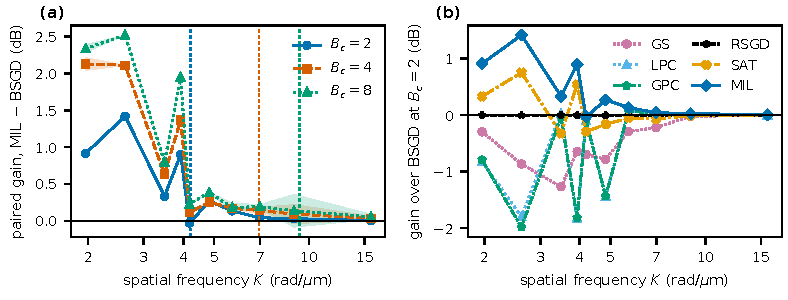
\includegraphics[width=\linewidth]{../code/figures/paper/Fig1_paired_gain.pdf}
\caption{(a) Paired gain (MIL $-$ BSGD) versus spatial frequency for three
contrast budgets; shading, 95\% $t$-intervals over three seeds; dashed lines,
heuristic $K_c(B_c)$ from Eq.~\eqref{eq:hk}. (b) Gain of every non-oracle
method over BSGD at $B_c=2$ (seed means); RSGD coincides with BSGD.}
\label{fig:gain}
\end{figure*}

Figure~\ref{fig:recon} shows single-seed reconstructions at the three $K$ of
the ablation studies; Supplement 1, Fig.~S1, shows the corresponding exposures
and index profiles. At the lowest $K$ MIL recovers most of the bar contrast
that BSGD loses; at the highest, both reconstructions are similarly shallow.

\begin{figure*}[!t]
\centering
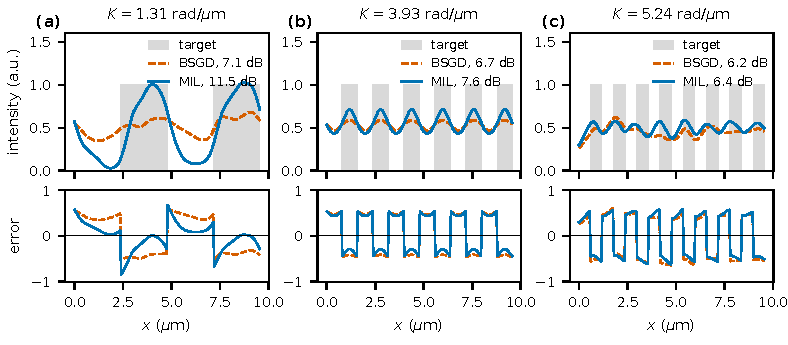
\includegraphics[width=\linewidth]{../code/figures/paper/Fig2_reconstructions.pdf}
\caption{Target, BSGD and MIL reconstructions (top) and errors (bottom) at
$B_c=2$, seed \ROneSeedValue, over a $9.6\,\mu$m section of the window;
legends give $\mathrm{PSNR}_{\text{si}}$. Single-seed illustrations;
Fig.~\ref{fig:gain} carries the statistics.}
\label{fig:recon}
\end{figure*}

Figure~\ref{fig:regime}(a) maps the same \MOneNCells{} cells as a single
picture, and its practical reading is that the benefit is concentrated at the
low-frequency, high-budget corner. A larger contrast budget buys more, and a
higher spatial frequency takes it away: the advantage is substantial below
about $3$\,rad/\textmu m and is not resolved from zero at the two highest $K$
at $B_c=4$ and 8.

\subsection{How much material a media-blind design wastes}
\label{sec:failure-rate}
Each exposure of a write-once medium consumes material, so average quality is
the wrong figure of merit on its own: what matters to a laboratory is how often
a recording comes out far worse than it needed to. An exposure fails if its
PSNR is more than a threshold below the constrained oracle's in the same cell
(Table~\ref{tab:failure-rate}; the \WastedMediaThreshDB\,dB threshold was fixed
before the results were computed). At \WastedMediaThreshDB\,dB,
\WastedMediaBSGDFrac\% of BSGD cells and \WastedMediaMILFrac\% of MIL cells
fail, and at \param{3}\,dB \WastedMediaBSGDFracThreeDB\% and
\WastedMediaMILFracThreeDB\%; at \param{1}\,dB the rates are similar
(\WastedMediaBSGDFracOneDB\% and \WastedMediaMILFracOneDB\%). MIL removes the
large shortfalls, not the small ones, which is the shape of benefit that
matters when each attempt costs a film. The rates are relative to a numerical
reference over \WastedMediaNConfigs{} cells, not to a proven optimum or over
physical trials.

\begin{table}[!htbp]
\centering
\caption{Failure rate: percentage of the \WastedMediaNConfigs{} grid cells in
which a method's seed-mean PSNR is more than the column threshold below the
constrained oracle's.}
\label{tab:failure-rate}
\begin{tabular}{lccccccc}
\hline
Threshold & GS & LPC & GPC & BSGD & RSGD & SAT & MIL \\
\hline
\param{1}\,dB & \WastedMediaGSFracOneDB & \WastedMediaLPCFracOneDB & \WastedMediaGPCFracOneDB & \WastedMediaBSGDFracOneDB & \WastedMediaRSGDFracOneDB & \WastedMediaSATFracOneDB & \WastedMediaMILFracOneDB \\
\WastedMediaThreshDB\,dB & \WastedMediaGSFrac & \WastedMediaLPCFrac & \WastedMediaGPCFrac & \WastedMediaBSGDFrac & \WastedMediaRSGDFrac & \WastedMediaSATFrac & \WastedMediaMILFrac \\
\param{3}\,dB & \WastedMediaGSFracThreeDB & \WastedMediaLPCFracThreeDB & \WastedMediaGPCFracThreeDB & \WastedMediaBSGDFracThreeDB & \WastedMediaRSGDFracThreeDB & \WastedMediaSATFracThreeDB & \WastedMediaMILFracThreeDB \\
\hline
\end{tabular}
\end{table}

\subsection{Simpler alternatives, and why they are not enough}
\label{sec:baselines}
At $B_c=2$ (Fig.~\ref{fig:gain}(b)), GS (\GSGainMin{} to \GSGainMax\,dB)
never improves on BSGD and LPC (\LPCGainMin{} to \LPCGainMax\,dB) improves on
it by at most \LPCGainMax\,dB; GPC (\GPCGainMin{} to \GPCGainMax\,dB) differs
from LPC by at most \GPCLPCMaxAbsDiffTwoX\,dB, consistent with both hitting
the same contrast clip. LPC is the closed-form use of Eq.~\eqref{eq:hk}, so its
failure is further evidence that the small-signal picture does not describe
this regime.

The saturation-only surrogate tests whether a laboratory could model the dose
response and ignore transport. Averaged over $K$, its gain is
\SATFracOfMILTwoX\%, \SATFracOfMILFourX\% and \SATFracOfMILEightX\% of MIL's at
$B_c=2$, 4 and 8, and by cell it recovers \SATFracLowKMin--\SATFracLowKMax\% of
MIL's gain at $K=1.96$\,rad/\textmu m and
\SATFracSecondKMin--\SATFracSecondKMax\% at $K=2.62$\,rad/\textmu m but scores
below BSGD in \SATNBelowBSGD{} of the \SATNCells{} cells where the ratio is
defined. A pointwise surrogate is therefore usable only at the lowest spatial
frequencies; elsewhere the full recording model is needed for any gain at all.

\subsection{Compute-matched control}
\label{sec:compute-matched}
MIL's per-iteration cost is about \ComputeMatchRatio$\times$ that of BSGD (one
wall-clock measurement), so a fair question is whether the baseline simply
needed longer. With \ComputeMatchRatio$\times$ more BSGD iterations at the
three ablation $K$ the paired gain is \MTwoRGainSub{} [\MTwoRLoSub,
\MTwoRHiSub], \MTwoRGainNear{} [\MTwoRLoNear, \MTwoRHiNear] and
\MTwoRGainPost\,dB [\MTwoRLoPost, \MTwoRHiPost], against \SOneGBaselineSub,
\SOneGBaselineNear{} and \SOneGBaselinePost\,dB at equal iteration count: the
extra iterations narrow the gap at the two lower $K$ but it stays positive at
all three. Wall-clock time is a noisy proxy for compute, so this tests a much
larger baseline budget rather than an equal-FLOP comparison.

\subsection{Which recording nonlinearity produces the gain}
\label{sec:mechanism}
Removing one mechanism at a time (Table~\ref{tab:mechanism}, top) leaves a
positive gain at every $K$, and which removal matters depends on $K$:
linearizing the index map raises the gain at $K=\SOneKSub$ and \SOneKPost{}
but lowers it at \SOneKNear\,rad/\textmu m. Because three mechanisms saturate
the dose response, removing one leaves the others, so we also ran all $2^3$
on/off combinations of monomer depletion (removed by holding $u=1$), dye
bleaching ($k_{\text{bleach}}=0$) and the $\tanh$ map, at a matched operating
point (Table~\ref{tab:mechanism}, bottom; all twelve conditions, including the
unmatched ones, in Supplement 1, Section S2). Removing monomer depletion at
fixed $\kappa$ raises the polymer cured by unit dose from $N\approx1$ to
$N\approx8.7$, so these conditions are run with $\kappa$ rescaled to restore
$N(E{=}1)=1$. A final control removes all three and sets
$\kappa=1/(1.5\,t_{\text{total}})$, which makes the recording BSGD's own linear
model up to non-local blur and shrinkage. The factorial ran on CPU and
reproduces the GPU full-model values to within \SXDeviceMaxDiff\,dB.

\begin{table}[!htbp]
\centering
\caption{Paired gain (dB) under mechanism ablations, $B_c=2$, mean of three
seeds. Top: one mechanism removed. Bottom: saturating mechanisms isolated at a
matched operating point, $N(E{=}1)=1$, and the slope-matched linear control;
blur, diffusion and shrinkage are kept. Intervals: Supplement 1, Figs.~S2--S3.}
\label{tab:mechanism}
\small\renewcommand{\arraystretch}{1.2}
\begin{tabular}{lccc}
\hline
Condition & $K=\SOneKSub$ & $K=\SOneKNear$ & $K=\SOneKPost$ \\
\hline
Full model & \SOneGBaselineSub & \SOneGBaselineNear & \SOneGBaselinePost \\
No non-locality ($\sigma=0$) & \SOneGNoNonlocSub & \SOneGNoNonlocNear & \SOneGNoNonlocPost \\
No diffusion ($D_0=0$) & \SOneGNoDiffSub & \SOneGNoDiffNear & \SOneGNoDiffPost \\
No dye bleaching ($k_{\text{bleach}}=0$) & \SOneGNoDyeSub & \SOneGNoDyeNear & \SOneGNoDyePost \\
No index saturation ($\tanh$ linearized) & \SOneGNoSatSub & \SOneGNoSatNear & \SOneGNoSatPost \\
\hline
Only monomer depletion & \SXGOnlyMonomerSub & \SXGOnlyMonomerNear & \SXGOnlyMonomerPost \\
Only dye bleaching & \SXGOnlyDyeMatchedSub & \SXGOnlyDyeMatchedNear & \SXGOnlyDyeMatchedPost \\
Only $\tanh$ map & \SXGOnlyTanhMatchedSub & \SXGOnlyTanhMatchedNear & \SXGOnlyTanhMatchedPost \\
Dye bleaching and $\tanh$ map & \SXGNoMonomerMatchedSub & \SXGNoMonomerMatchedNear & \SXGNoMonomerMatchedPost \\
Linear, slope-matched & \SXGLinearMatchedSub & \SXGLinearMatchedNear & \SXGLinearMatchedPost \\
\hline
\end{tabular}
\end{table}

Three observations follow. First, when the recording is the media-blind model
up to blur and shrinkage, MIL gains essentially nothing at the two lower $K$, so
the gain there requires a nonlinear dose response; at $K=\SOneKPost$\,rad/\textmu m
the linear control's gain (\SXGLinearMatchedPost\,dB) is comparable to the full
model's (\SOneGBaselinePost\,dB), so the small gain there may come from the blur
and shrinkage that BSGD ignores. Second, each saturating mechanism alone
produces a gain at the two lower $K$, so no single mechanism is necessary.
Third, monomer depletion alone gives a larger gain than the full model at every
$K$, so the mechanisms' effects do not add. For a laboratory this is the
encouraging result: the method does not require identifying which
nonlinearity a given medium has, only that it has one and that the model
captures it. The matching criterion $N(E{=}1)=1$ is our choice; another
normalization could reorder the single mechanisms, though not the null result of
the linear control.

\subsection{Where it fails: fringe slant}
\label{sec:slant}
Every result above is for an unslanted grating, and that restriction is not a
convenience. With everything else fixed, the paired gain depends strongly and
non-monotonically on the fringe slant $\phi$ (Fig.~\ref{fig:regime}(b);
Supplement 1, Section S3). At $\phi=0^\circ$, $5^\circ$, $10^\circ$ and
$20^\circ$ it is \SEightGainKLowSlantZero, \SEightGainKLowSlantFive,
\SEightGainKLowSlantTen{} and \SEightGainKLowSlantTwenty\,dB at
$K=1.96$\,rad/\textmu m and \SEightGainKMidSlantZero,
\SEightGainKMidSlantFive, \SEightGainKMidSlantTen{} and
\SEightGainKMidSlantTwenty\,dB at $K=\SOneKNear$\,rad/\textmu m. Small slants
appear to increase the gain; from $\phi=\SlantCollapseDeg^\circ$ onwards it has
collapsed at both tested $K$, with no value above
\SlantMaxGainBeyondCollapse\,dB at any larger angle.

\textbf{Mechanism.} The collapse is Bragg detuning, not a failure of the
exposure design. Over a grid of \RCWASlantNCases{} RCWA cases spanning the
tested $K$, three index-modulation levels, both polarizations and both
incidence conventions, the first-order transmitted efficiency at Bragg
incidence falls from \RCWASlantFirstZero{} at $\phi=0^\circ$ to
\RCWASlantFirstTwoFive{} at $\phi=2.5^\circ$ and
\RCWASlantFirstTwenty{} at $20^\circ$, while the undiffracted order rises from
\RCWASlantZerothZero{} to \RCWASlantZerothTwenty{}
(Fig.~\ref{fig:regime}(c)). Tilting the fringes rotates the grating vector out
of the symmetric two-wave geometry, so at a fixed readout angle the grating
simply stops diffracting. Once the reconstruction is carried by the
undiffracted beam, there is nothing left for any exposure design to improve and
the paired difference between two designs goes to zero. The angular scale is
the grating's own selectivity, of order $\Lambda/T$, which is $6.1^\circ$ at
$K=1.96$ and $3.1^\circ$ at $K=\SOneKNear$\,rad/\textmu m.

\textbf{Why the apparent enhancement is not reported as one.} The same sweep
shows that the closed-form readout reference loses validity at the first
nonzero tested angle: the median deviation of Kogelnik theory from RCWA jumps
from \RCWASlantDevZero{} at $\phi=0^\circ$ to \RCWASlantDevTwoFive{} at
$\phi=\RCWASlantOnsetDeg^\circ$ and stays there. The peak in
Fig.~\ref{fig:regime}(b) at $2.5$ to $5^\circ$ therefore sits entirely inside
the range where the closed form is already wrong by about half the available
efficiency, and the split-step readout in the design loop shares its scalar
paraxial approximation and has not itself been checked against RCWA at slant.
We therefore state the validated envelope as unslanted gratings only, and treat
both the apparent enhancement at small slant and the exact collapse angle as
model-dependent. The useful design statement is the conservative one: do not
expect this method to help a slanted hologram on the strength of these results.

\begin{figure*}[!t]
\centering
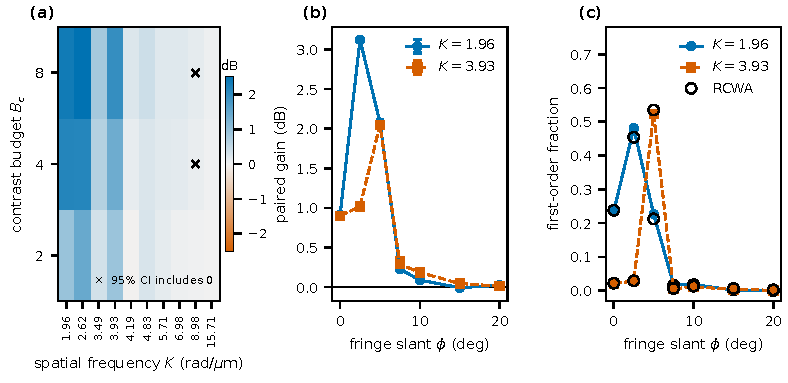
\includegraphics[width=\linewidth]{../code/figures/paper/Fig3_regime_map.pdf}
\caption{Operating regime. (a) Paired gain over the \MOneNCells{} grid cells;
crosses mark cells whose 95\% interval includes zero. (b) Paired gain versus
fringe slant at two $K$, $B_c=2$, 95\% $t$-intervals over three seeds; the
shaded region is where the readout has not been checked against RCWA. (c)
Median RCWA transmitted efficiency at Bragg incidence over the same slant grid:
the diffracted order collapses as soon as the fringes tilt.}
\label{fig:regime}
\end{figure*}

\subsection{Robustness to twin miscalibration}
\label{sec:robustness}
\textbf{One parameter.} Here both exposures are designed once with the nominal
parameters and recorded, without re-optimization, on a twin with $D_0$,
$\sigma$, $\kappa$ or $\Delta n_{\max}$ perturbed by $\pm10$, $\pm25$ or
$\pm50\%$ (Supplement 1, Section S4 and Fig.~S6). BSGD's design uses no
recording parameter (only $\Delta n_{\max}$, as the scale of its linear model),
so the test measures how much MIL's advantage depends on a correct twin. The
$K$-averaged gain ranges from \SThreeWorstWithinFifty{} to
\SThreeBestWithinFifty\,dB (nominal \SThreeNominalGain\,dB). We swept
$\Delta n_{\max}$ further because two fits of the twin to Bayfol HX data
disagree on it by \BayfolDnMaxRatio$\times$ (Section~\ref{sec:twin-validation}):
the gain is \SThreeDnMaxAtMostNegative\,dB at
$\SThreeDnMaxMostNegativePct\%$, \SThreeDnMaxAtPlusFifty\,dB at $+50\%$,
\SThreeDnMaxAtHundred\,dB at $+100\%$ and \SThreeDnMaxAtMostPositive\,dB at
$+\SThreeDnMaxMostPositivePct\%$. A twin that underestimates the medium's
index budget several-fold can therefore make MIL worse than the media-blind
baseline; where between $+100\%$ and $+\SThreeDnMaxMostPositivePct\%$ the sign
changes was not resolved.

\textbf{Joint and structural errors.} In \SSixNDraws{} Monte Carlo draws with
all four parameters perturbed independently and uniformly within
$\pm$\SSixPctRange\% (same designed exposures), the $K$-averaged gain ranges from
\SSixWorstDrawGain{} to \SSixBestDrawGain\,dB (mean \SSixMeanGain\,dB,
bootstrap 95\% interval [\SSixBootCILo, \SSixBootCIHi]); \SSixNNegative{} of
\SSixNDraws{} are negative. Beer--Lambert attenuation through depth (16 recorded
slices) gives \SSevenGainODZero, \SSevenGainODOneTenth{} and
\SSevenGainODThreeTenths\,dB at optical density 0, 0.1 and 0.3. Re-optimizing
both arms on media with $D_0$, $\sigma$ or $\kappa$ changed by up to $\pm50\%$
($K=\SOneKPost$\,rad/\textmu m) gives \STwoGainMin{} to \STwoGainMax\,dB
(nominal \STwoBaselineGain\,dB).

\textbf{Targets and noise.} At $K=\SOneKNear$\,rad/\textmu m and $B_c=2$ the
gain is \SFourGainBarsTwoX{} for bars, \SFourGainSpotsTwoX{} for sparse random
spots and \SFourGainRandomBinaryTwoX\,dB for a random binary target, and
Gaussian detector noise at \SFiveNoiseStdPct\% of the peak changes the bar
gain from \SFiveNoiselessGain{} to \SFiveNoisyGain\,dB (Supplement 1,
Section S8).

\subsection{Which parameter has to be right}
\label{sec:sensitivity}
Robustness over a range is not the same as knowing which measurement to make
carefully, so we rank the four recording parameters by how much the gain moves
when each is wrong (Fig.~\ref{fig:sens}). Two independent views agree on the
order.

One at a time (Fig.~\ref{fig:sens}(a)), the $K$-averaged gain spans
\SensRangeDnMax\,dB as $\Delta n_{\max}$ alone moves over $\pm50\%$, against
\SensRangeKappa\,dB for $\kappa$, \SensRangeDZero\,dB for $D_0$ and
\SensRangeSigma\,dB for $\sigma$, from a nominal \SensNominalGain\,dB. The
index budget therefore outranks the next parameter by
\SensTopRangeRatio$\times$, and its worst case is an underestimate: at
$\SensWorstPctDnMax\%$ the gain falls to \SensWorstDnMax\,dB. For $D_0$ the
worst case is an overestimate ($\SensWorstPctDZero\%$); for $\kappa$ and
$\sigma$ it is an underestimate.

Across the \SensNDraws{} joint draws (Fig.~\ref{fig:sens}(b)), regressing the
per-draw gain on the four standardized errors gives
\SensBetaDnMax\,dB per standard deviation for $\Delta n_{\max}$
[\SensBetaLoDnMax, \SensBetaHiDnMax], \SensBetaKappa{} for $\kappa$
[\SensBetaLoKappa, \SensBetaHiKappa], \SensBetaDZero{} for $D_0$
[\SensBetaLoDZero, \SensBetaHiDZero] and \SensBetaSigma{} for $\sigma$
[\SensBetaLoSigma, \SensBetaHiSigma]; \SensNResolved{} of the four intervals
exclude zero, $\sigma$ being the one that does not. The linear terms account
for $R^2=\SensRSquared$ of the spread across draws. With this many draws the
interaction and higher-order terms are not identifiable, so this is a
first-order attribution over the tested $\pm$\SSixPctRange\% box, not a Sobol
decomposition; the rank order, not the coefficient values, is what we rely on.

\begin{figure*}[!t]
\centering
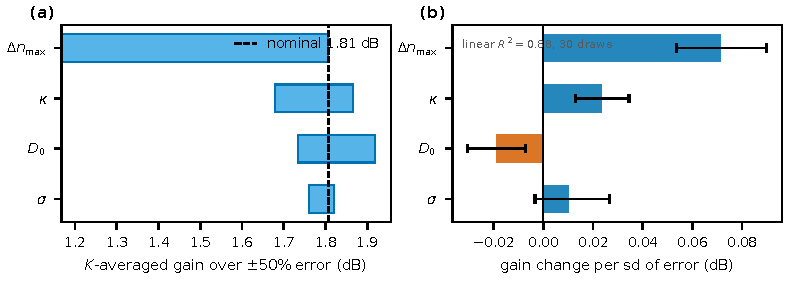
\includegraphics[width=\linewidth]{../code/figures/paper/Fig4_sensitivity.pdf}
\caption{Parameter sensitivity of the design gain. (a) Span of $K$-averaged
paired gain covered as each parameter alone is varied over $\pm50\%$, against
the nominal value (dashed). The worst case is the $-50\%$ end for
$\Delta n_{\max}$, $\kappa$ and $\sigma$ and the $+50\%$ end for $D_0$. (b)
Gain change per standard deviation of each parameter's error across
\SensNDraws{} joint draws, with bootstrap 95\% intervals; colour marks sign.
Rows are in the same order in both panels.}
\label{fig:sens}
\end{figure*}

\section{Twin validation against published data}
\label{sec:twin-validation}
We fit the twin to the first-harmonic index modulation $\Delta n_1$ versus
dose in Fig.~3 of Bruder et al.~\cite{bruder2017bayfol} (Bayfol HX,
$\Lambda=700$\,nm, $K=8.98$\,rad/\textmu m, inside the tested grid): the
source's kinetic-model curve (16.7\,mW/cm$^2$) and its measurement
(19.2\,mW/cm$^2$), read visually rather than with a calibrated digitizer (about
$\pm10\%$ in dose, $\pm3$--$5\%$ in $\Delta n_1$). Unfitted parameters take
Bayfol HX values from the released configuration; each fit is the best of 8--10
random starts, and NRMSE is the root-mean-square residual over the range of the
fitted data.

\textbf{Fits and held-out prediction.} With $\kappa$, $\Delta n_{\max}$ and
$k_{\text{bleach}}$ free, the twin reproduces the rise-then-decline shape of
both series (Fig.~\ref{fig:twin}; in-sample NRMSE \HoldoutBSimIn{} for the
model curve, \HoldoutBExpIn{} for the measurement). Both are plotted against
dose and the twin is dose-reciprocal at $\gamma=1$, so a fit to one series
predicts the other without refitting, with NRMSE \HoldoutBSimOut{} (model to
measurement) and \HoldoutBExpOut{} (the reverse). The fitted
$k_{\text{bleach}}$ are \HoldoutBSimKbleach{} and \HoldoutBExpKbleach{} (default
0.2) and the fitted $\Delta n_{\max}$ \HoldoutBSimDnMax{} and
\HoldoutBExpDnMax. With $k_{\text{bleach}}$ held at 0.2 the in-sample NRMSE is
\NRMSEBruderGrowthDnKSim{} and \NRMSEBruderGrowthDnKExp, but the measured-series
optimum is degenerate (its $\kappa$ saturates the medium before the first
measured dose, giving an almost constant $\Delta n_1$; Supplement 1, Fig.~S5),
the held-out NRMSEs are \HoldoutASimOut{} and \HoldoutAExpOut, and the fitted
$\Delta n_{\max}$ disagree by \BayfolDnMaxRatio$\times$, which sets the range of
the $\Delta n_{\max}$ sweep in Section~\ref{sec:robustness}. Fig.~S5 also shows
a fit to a PQ/PMMA $\Delta n_1(t)$ model curve~\cite{hsieh2022pqpmma} outside
the tested $K$ range (NRMSE \NRMSEHsiehGrowthDnK).

\begin{figure*}[!t]
\centering
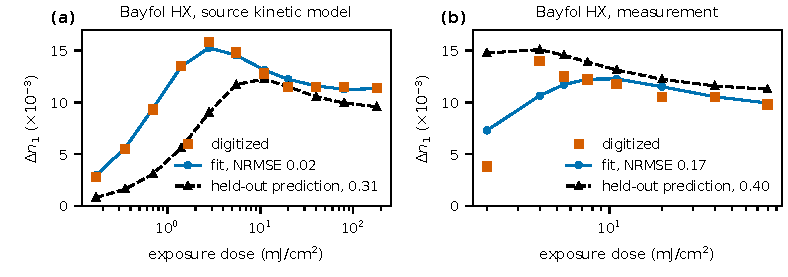
\includegraphics[width=\linewidth]{../code/figures/paper/Fig5_twin_validation.pdf}
\caption{Twin fitted to $\Delta n_1$ digitized from Bruder et
al.~\cite{bruder2017bayfol} (Bayfol HX): (a) the source's kinetic-model curve,
(b) its measurement. Solid, fit to the series shown ($\kappa$,
$\Delta n_{\max}$, $k_{\text{bleach}}$ free); dashed, parameter-free
prediction from the fit to the other series. Legends give NRMSE.}
\label{fig:twin}
\end{figure*}

\textbf{What this establishes, and what it does not.} The model family can
reproduce, and predict across two views of the same condition, the dose
response of one commercial photopolymer with effective parameters. It does not
pin the default medium of Table~\ref{tab:mediumparams} to a real material or
test transfer across $K$ or media: the two series share a material, a grating
and nearly the same intensity, and one is a model output. $D_0$ and $\sigma$
are identifiable only from multi-$K$ growth-curve families, which we did not
have; Section~\ref{sec:guidelines} states what to measure instead. The headline
claims therefore rest on the paired design and the miscalibration tests, not on
absolute agreement with a real medium.

\section{Design guidelines and calibration protocol}
\label{sec:guidelines}
This section is the operational summary: what a laboratory would measure,
in what order, and when not to bother.

\textbf{Step 1: decide whether the geometry qualifies.} Use the method for
unslanted transmission gratings only. The gain collapses from
$\phi=\SlantCollapseDeg^\circ$ and the readout is unvalidated at any nonzero
slant (Section~\ref{sec:slant}). Within that geometry, read
Fig.~\ref{fig:regime}(a): the benefit is concentrated below about
$3$\,rad/\textmu m and grows with the contrast budget the setup can deliver. At
the top of the tested range the gain is under \GainHighKEightX\,dB and not
worth the calibration effort.

\textbf{Step 2: measure the dose response at the working point.} One
$\Delta n_1$ versus dose curve, recorded at the spatial frequency and intensity
the application will use, identifies $\kappa$ and $\Delta n_{\max}$. Fit
$k_{\text{bleach}}$ jointly rather than assuming it: holding it at a nominal
value made our own fit degenerate, with $\kappa$ saturating the medium before
the first measured dose (Supplement 1, Section S9). Take $\Delta n_{\max}$ from
the same experimental condition as the curve being fitted, never from a
separate experiment on nominally the same material; two fits that differ in
this respect disagreed by \BayfolDnMaxRatio$\times$
(Section~\ref{sec:twin-validation}).

\textbf{Step 3: measure at more than one spatial frequency.} $D_0$ and
$\sigma$ act only through the spatial-frequency dependence, so a single-$K$
curve cannot identify them and should not be used to try. A growth-curve family
at three or more spatial frequencies spanning the intended operating range, or
an independent measurement of monomer diffusivity, is the minimum. Thickness
and shrinkage are measured separately by angular scan.

\textbf{Step 4: spend the effort where it matters.} The ranking of
Section~\ref{sec:sensitivity} is unambiguous: $\Delta n_{\max}$ dominates,
outranking $\kappa$ by \SensTopRangeRatio$\times$ and $\sigma$ by more than an
order of magnitude. A $50\%$ underestimate of the index budget costs
\SensRangeDnMax\,dB of the \SensNominalGain\,dB nominal gain, and a
several-fold underestimate reverses the sign of the benefit entirely
(Section~\ref{sec:robustness}). An error in $\sigma$, by contrast, is the one
whose effect is not resolved from zero across the joint draws. If calibration
time is limited, spend it on the index budget and the dose response, not on the
non-local length.

\textbf{Step 5: budget the compute.} Designing through the model cost about
\ComputeMatchRatio$\times$ per iteration here, and the advantage survives giving
the media-blind baseline that factor more iterations
(Section~\ref{sec:compute-matched}). At the grid size used, a design is minutes
on a laptop GPU, which is small against the cost of a wasted film.

\textbf{When not to use the method.} If the fringes are slanted; if the target
spatial frequency is at the top of the tested range; if $\Delta n_{\max}$ is
not known to better than a factor of two under the recording condition; or if
the application sits at the very lowest spatial frequencies and a calibrated
pointwise saturating model is already available, since that surrogate recovers
\SATFracLowKMin--\SATFracLowKMax\% of the gain there
(Section~\ref{sec:baselines}) for a fraction of the modelling effort.

\section{Limitations}
\label{sec:discussion}
\textbf{No physical recording.} All results are simulation outputs of one model
family. Whether the gains transfer to a physical photopolymer is untested; the
decisive experiment, recording optimized and media-blind exposures in a
characterized medium and comparing the measured reconstructions, is future
work. What the multi-parameter miscalibration and sensitivity studies do cover
is the question a laboratory would ask next: how wrong the model can be before
the benefit disappears, and which parameter that depends on.

\textbf{Validation breadth.} The twin is compared with one commercial medium at
one spatial frequency, in two views of the same recording condition, one of
which is itself a model output, and the points were read visually rather than
with a calibrated digitizer. Transfer across $K$ and across media is untested,
which is exactly the measurement Step~3 of Section~\ref{sec:guidelines} asks a
calibrating laboratory to make.

\textbf{Geometry and targets.} One-dimensional transverse recording of binary
bar targets in unslanted gratings, with one default medium and three seeds per
cell. Against RCWA~\cite{moharam1981rigorous} (computed with
TORCWA~\cite{kim2023torcwa}) over a \RCWAVGridNCases-case grid of $K$,
$\Delta n$, polarization and slant, Kogelnik theory deviates by at most
\RCWAUnslantedMaxDev{} in diffraction efficiency for unslanted geometries but
by up to \RCWAVGridMaxDev{} at a $20^\circ$ slant (Supplement 1, Section S5),
and the slant sweep of Section~\ref{sec:slant} shows that departure setting in
at the smallest nonzero angle tested. The check concerns the closed-form
reference; the beam propagation in the design loop shares its paraxial scalar
approximation and was not separately checked against RCWA at slant.

\textbf{Model and statistics.} The recorded profile is uniform through depth
except in the Beer--Lambert check; diffusion uses a spatially averaged
coefficient; the index map and its shape constant are modelling choices;
shrinkage is a placeholder; the medium parameters are illustrative; and the
factorial covers interactions among the saturating mechanisms only. Three
seeds per cell measure initialization sensitivity, which is small here; model
and parameter error are probed only by the miscalibration and sensitivity
studies over the stated ranges. The \MOneNK-point grid does not resolve
features between grid points, such as the zero crossing at $B_c=2$.

\section{Conclusion}
\label{sec:conclusion}
In simulation, designing the exposure of a write-once volume photopolymer
through a differentiable NPDD and beam-propagation model improves on
media-blind design in \MOneNPositive{} of \MOneNCells{} unslanted grating
cells, by up to \MaxGainEightX\,dB at low spatial frequency, and removes the
exposures that fall more than \WastedMediaThreshDB\,dB short of an oracle
reference. The gain requires a nonlinear dose response but no particular
saturating mechanism, which means a laboratory need not identify its medium's
nonlinearity, only model it. It decays toward zero at high spatial frequency,
survives joint parameter errors of $\pm$\SSixPctRange\%, and depends above all
on the recorded index budget $\Delta n_{\max}$, a several-fold underestimate of
which reverses the benefit. It collapses once the fringes tilt, for a reason
that is optical rather than algorithmic: a slanted grating stops diffracting at
a fixed readout angle. The calibration protocol of
Section~\ref{sec:guidelines} states the minimum measurement set; testing these
predictions in a recorded medium is the next step.

\begin{backmatter}

\bmsection{Funding}
This research received no external funding.

\bmsection{Acknowledgment}
The author used Claude (Anthropic; Claude Code with the Claude Sonnet 5 and
Claude Opus 4.8, 5 and 5.5 models) to write and debug simulation and analysis
code, to read the data points digitized in Section~\ref{sec:twin-validation},
and to draft and edit the text; the author reviewed all outputs and takes full
responsibility for the content.

\bmsection{Disclosures}
The author declares no conflicts of interest.

\bmsection{Data availability}
Code, experiment manifests, raw per-job result files and the scripts that
generate every number and figure in this paper are available on GitHub
(\url{https://github.com/ultramagnus23/HoloForge}) and archived in
Ref.~\cite{holoforge2026code}.

\bmsection{Supplemental document}
See Supplement 1 for supporting content.

\end{backmatter}

\bibliography{refs}

\end{document}
